%
% This is the LaTeX template file for lecture notes for EE 382C/EE 361C.
%
% To familiarize yourself with this template, the body contains
% some examples of its use.  Look them over.  Then you can
% run LaTeX on this file.  After you have LaTeXed this file then
% you can look over the result either by printing it out with
% dvips or using xdvi.
%
% This template is based on the template for Prof. Sinclair's CS 270.

\documentclass[twoside]{article}
\usepackage{graphics}
\usepackage{tikz}
\usepackage{listings}
\usepackage{graphicx}
\usepackage{float}
\graphicspath{ {images/} }
\usetikzlibrary{arrows,positioning,automata,shadows,fit,shapes}
\setlength{\oddsidemargin}{0.25 in}
\setlength{\evensidemargin}{-0.25 in}
\setlength{\topmargin}{-0.6 in}
\setlength{\textwidth}{6.5 in}
\setlength{\textheight}{8.5 in}
\setlength{\headsep}{0.75 in}
\setlength{\parindent}{0 in}
\setlength{\parskip}{0.1 in}

%
% The following commands set up the lecnum (lecture number)
% counter and make various numbering schemes work relative
% to the lecture number.
%
\newcounter{lecnum}
\renewcommand{\thepage}{\thelecnum-\arabic{page}}
\renewcommand{\thesection}{\thelecnum.\arabic{section}}
\renewcommand{\theequation}{\thelecnum.\arabic{equation}}
\renewcommand{\thefigure}{\thelecnum.\arabic{figure}}
\renewcommand{\thetable}{\thelecnum.\arabic{table}}

%
% The following macro is used to generate the header.
%
\newcommand{\lecture}[4]{
   \pagestyle{myheadings}
   \thispagestyle{plain}
   \newpage
   \setcounter{lecnum}{#1}
   \setcounter{page}{1}
   \noindent
   \begin{center}
   \framebox{
      \vbox{\vspace{2mm}
    \hbox to 6.28in { {\bf EE 382C/361C: Multicore Computing
                        \hfill Fall 2016} }
       \vspace{4mm}
       \hbox to 6.28in { {\Large \hfill Lecture #1: #2  \hfill} }
       \vspace{2mm}
       \hbox to 6.28in { {\it Lecturer: #3 \hfill Scribe: #4} }
      \vspace{2mm}}
   }
   \end{center}
   \markboth{Lecture #1: #2}{Lecture #1: #2}
   %{\bf Disclaimer}: {\it These notes have not been subjected to the
   %usual scrutiny reserved for formal publications.  They may be distributed
   %outside this class only with the permission of the Instructor.}
   \vspace*{4mm}
}

%
% Convention for citations is authors' initials followed by the year.
% For example, to cite a paper by Leighton and Maggs you would type
% \cite{LM89}, and to cite a paper by Strassen you would type \cite{S69}.
% (To avoid bibliography problems, for now we redefine the \cite command.)
% Also commands that create a suitable format for the reference list.
\renewcommand{\cite}[1]{[#1]}
\def\beginrefs{\begin{list}%
        {[\arabic{equation}]}{\usecounter{equation}
         \setlength{\leftmargin}{2.0truecm}\setlength{\labelsep}{0.4truecm}%
         \setlength{\labelwidth}{1.6truecm}}}
\def\endrefs{\end{list}}
\def\bibentry#1{\item[\hbox{[#1]}]}

%Use this command for a figure; it puts a figure in wherever you want it.
%usage: \fig{NUMBER}{SPACE-IN-INCHES}{CAPTION}
\newcommand{\fig}[3]{
			\vspace{#2}
			\begin{center}
			Figure \thelecnum.#1:~#3
			\end{center}
	}
% Use these for theorems, lemmas, proofs, etc.
\newtheorem{theorem}{Theorem}[lecnum]
\newtheorem{lemma}[theorem]{Lemma}
\newtheorem{proposition}[theorem]{Proposition}
\newtheorem{claim}[theorem]{Claim}
\newtheorem{corollary}[theorem]{Corollary}
\newtheorem{definition}[theorem]{Definition}
\newenvironment{proof}{{\bf Proof:}}{\hfill\rule{2mm}{2mm}}

% **** IF YOU WANT TO DEFINE ADDITIONAL MACROS FOR YOURSELF, PUT THEM HERE:

\begin{document}
%FILL IN THE RIGHT INFO.
%\lecture{**LECTURE-NUMBER**}{**DATE**}{**LECTURER**}{**SCRIBE**}
\lecture{13}{October 11}{Vijay Garg}{Harsh Yadav}
%\footnotetext{These notes are partially based on those of Nigel Mansell.}

% **** YOUR NOTES GO HERE:

% Some general latex examples and examples making use of the
% macros follow.  
%**** IN GENERAL, BE BRIEF. LONG SCRIBE NOTES, NO MATTER HOW WELL WRITTEN,
%**** ARE NEVER READ BY ANYBODY.
\section*{Agenda}
The lecture focused on Concurrent Data Structures. Chapter-5 (Wait Free Synchronization) will be continued on next class meeting. Major concepts discussed -:
\begin{itemize}
    \item Classifications of Concurrent Data Structures
    \item Concurrent Stacks
    \item Concurrent Queues
    \item Concurrent Linked Lists
\end{itemize}

\section{Introduction}
A \textbf{Concurrent Data Structure} is a particular way of storing and organizing data for access by multiple computing threads (or processes) on a computer. 
Concurrent Data Structures are classified as following -:
\begin{center}
\begin{tikzpicture} %[scale=.6,transform shape] %<-- uncomment this to see the effect
\tikzstyle{level 1}=[sibling distance=52mm] 
\tikzstyle{level 2}=[sibling distance=30mm] 

 \node{Concurrent Data Structures} 
  child{node{Lock Based} 
     child{node{Coarse Grained}}
     child{node{Fine Grained}}
  } 
  child{node{Lock Free}
   child{node{Lock free}}
   child{node{Wait free}}
  }; 
 \end{tikzpicture}
\end{center}

The main difference between lock based and lock free implementation lies in the technique to enable mutual exclusion. Lock based primarily works on the concept of \textit{locking, mutually exclusive operation and then unlocking}. However, In lock-free, there is no explicit locking. The mutually exclusive operations happen using \textit{CAS - Compare and Set operation}. The process keeps on trying in a while loop until \textit{CAS} succeeds. \textit{CAS} acts as the linearization point in lock-free scheme. (\textit{Refer to AtomicInteger.Java for an example of lock-free using CAS on course github page}).

\textbf{\textit{Coarse Grained}} - It refers to locking at entry and unlocking at exit while using a data-structure.It is less efficient in terms of exploiting concurrency. It is relatively easier to implement and should be used when Data-structure is not in the critical path (Data Structure's performance is not of much significance).  

\textbf{\textit{Fine Grained}} - It refers to using multiple locks and implement a more finer locking scheme into various operations instead of explicitly locking at entry and unlocking at exit. (Difficult to implement)
\begin{center}
\renewcommand{\lstlistingname}{Code}
\begin{lstlisting}[language=Java, caption=Lock Free Implementation, frame=single, basicstyle=\Large]
int regularLockFreeOperation(){
    ...
    ...
    while(true){
        if(CAS(....)){
            return;
        }else{
            Thread.yield();
        }
    }    
}
\end{lstlisting}
\end{center}

\section{Concurrent Stacks}
The main operations associated with stacks are -:
\begin{itemize}
    \item \textbf{Push}
    \item \textbf{Pop}
\end{itemize}
The concurrent stack implementation is pretty straightforward.

\textbf{\textit{Lock Based}} - Lock based stack can be implemented by simple usage of monitors (\textit{Synchronized and Reentrant locks}) for \textit{push} and \textit{pop} operations.

\textbf{\textit{Lock free}} - Lock free stack implementation can be achieved by standard \textit{CAS} operation in a while loop as discussed in the previous section. (\textit{Refer to LockFreeStack.java on course github page})

\textit{NOTE} - One thing to note while doing lock-free implementations using above discussed technique is to make while() loop as tight as possible. (ex - Refrain from allocating memory inside the while() loop)

\textbf{\textit{Speedup trick for Lock-free Stack (Cancellation of Operations)}} - If there are concurrent push and pop operations happening on stack as shown in Fig 13.1, Stack can be made faster. As shown in the figure, only one of the \textit{push} operation will succeed (either \textit{push(70) or push(30)}).Let's say push(70) succeeded. As, there is a concurrent pop() operation happening, \textit{push(30)} can be cancelled by \textit{pop()} operation. In implementation, an Exchanger has to be implemented to keep record of all the operations and cancel them if a scenario like this exists.
\begin{figure}[H]
\centering
\includegraphics[scale=0.5]{Stack}
\caption{Concurrent Stack}
\label{fig:2}
\end{figure}

\section{Concurrent Queue}
The main operations associated with stacks are -:
\begin{itemize}
    \item \textbf{Enqueue}
    \item \textbf{Dequeue}
\end{itemize}
\begin{center}
\begin{tikzpicture} %[scale=.6,transform shape] %<-- uncomment this to see the effect
\tikzstyle{level 1}=[sibling distance=52mm] 
\tikzstyle{level 2}=[sibling distance=30mm] 

 \node{Concurrent Queue} 
  child{node{Bounded} 
     child{node{Blocking}}
     child{node{Non Blocking}}
  } 
  child{node{Unbounded}
   child{node{Blocking}}
   child{node{Non Blocking}}
  }; 
 \end{tikzpicture}
\end{center}
Each of the leaf nodes can be further classified into lock based and lock free.

\subsection{Lock Based}

Lock based implementation is usually achieved by using standard monitors. One tweak to fasten lock based implementations is to use multiple locks instead of using single lock. The reason why multiple locks are utilized here and not for Stacks is that operations are happening in queue at both ends \textit{(Enqueue - Tail, Dequeue - Head)} as opposed to Stack where both \textit{(Push and Pop)} operations were happening at the top of the stack. (\textit{Refer to UnboundedQueue.Java and unbounded-total-lock-based-queue.txt on course github page})

\textbf{NOTE} - Queue implementation can be made more faster by using the concept of \textit{Sentinel} node. As we know, In both \textit{Dequeue \& Enqueue} operations, we have to check first that the head is not null. The \textit{if} statement gets executed in multiple instructions at processor level. These checkings can be avoided if Queue is designed to have at-least one node, even when it is empty (\textit{Sentinel node}). One more thing that can be kept in mind for \textit{Dequeue} operation is to shift the sentinel node(head) to next node instead of pointing the old head to the next. The concep of \textit{Sentinel} node is more beneficial for Lock free implementation.

\subsection{No lock No CAS queue}
This is a special version of queue (bounded) which can be implemented without any Locks as well as without any CAS operations. The important thing to note here is this type of implementation can be done only for \textit{Single Consumer Single Producer} scenario (\textit{Refer to SingleQueue.Java on course github page}). Here \textit{put} is reading the value of \textit{head} and \textit{get} is reading the value of \textit{tail}. The consistency conditions on reading \textit{head \& tail} will give either the current value or the previous value depending on whether any concurrent operation is happening to update these registers or not. In both the cases, the legality of both \textit{put() \& get()} operations is maintained. It is impossible to make a Lock free and CAS free queue for multiple consumers or multiple producers scenario.
\begin{center}
\renewcommand{\lstlistingname}{Code}
\begin{lstlisting}[language=Java, caption=No Lock No CAS Queue, frame=single]
  public void put(Object x) {
    while (tail - head == items.length) {}; //busywait
    items[tail % items.length] = x;
    tail++;
  }
  public Object get() {
    while (tail - head == 0) {}; // busywait
    Object x = items[head % items.length];
    head++;
    return x;
  }
\end{lstlisting}
\end{center}

\subsection{Lock Free (Michael and Scott's Algorithm)}
The usual Lock free implementation uses CAS operation. One problem that may arise in lock-free queue using CAS operations is \textbf{ABA problem}.

\subsubsection{ABA problem}
 ABA problem occurs during synchronization, when a location is read twice, has the same value for both reads, and "value is the same" is used to indicate "nothing has changed". However, another thread can execute between the two reads and change the value, do other work, then change the value back, thus fooling the first thread into thinking "nothing has changed" even though the second thread did work that violates that assumption. Suppose a thread is in the process of swinging the \textit{tail} pointer from \textit{A} to \textit{P} (while enquing P) using a CAS operation. Before the CAS happens, another thread T1 comes and swings the pointer to B (B enqueued). Now, CAS fails in compare operation. Now memory location A is free. Suppose another thread comes and swings the Tail pointer to A (in a new enqueue operation). Now the previous CAS operation which failed in compare will succeed and behave as if nothing has changed which is not the case as there is a separate enqueue(B) which happened. Note that this condition is very rare as it is very less probability for a new enqueue operation to exactly use the same memory location (A) just after it got freed.
 \begin{figure}[H]
\centering
\includegraphics[scale=0.5]{ABA}
\caption{ABA problem}
\label{fig:2}
\end{figure}

\textbf{\textit{Solution}} - The solution to this problem was given by \textit{Michael and Scott}.The solution is based on attaching a number to the pointer and increment it every time the Tail is assigned to the pointer. In this way, CAS (which reads a complete word) will be able to identify that A is a different version while doing the CAS operation second time in the above discussed scenario.

\subsubsection{Helping} - Another feature given by \textit{Michael and Scott's} algorithm is \textit{helping}. As, In the lock-free scenario, the state of a process is visible, another process can take on the work of a process (who haven't finished yet) and finish it to speedup the execution.
In the M\&S imlementation, there are two CAS operations in the main loop \textit{(in both enqueue and dequeue)}. Lets take an instance of enqueue operation, the first CAS is trying to add a new node at the end of the linked list (Linked List implementation of queue). If first CAS is successful, enqueue is completed and process exits from the loop. If CAS is not successful, then the process tries to help some other process (2nd CAS operation in loop) which is in the middle of enqueue to swing tail to the next node (2nd CAS operation - idempotent). After that, the process starts again for its own enqueue.

\section{Concurrent Linked List}
The main operations associated with stacks are -:
\begin{itemize}
    \item \textbf{Add}
    \item \textbf{Remove}
    \item \textbf{Contains} - read only operation (should occur faster, avoid using locks in it)
\end{itemize}

 \begin{figure}[H]
\centering
\includegraphics[scale=0.8]{LL}
\caption{Linked List}
\label{fig:2}
\end{figure}

We need locks for implementing linked lists because any operation (Add and Remove) involves two nodes. If we are doing lock-free implementation, there may be instances when there is an Add operation going on and someone removes previous node. For example, there is an add operation going on for \textit{Node 3} and someone removes \textit{Node 0}, at this point \textit{Node 3} is lost. To prevent this kind of scenario, we need locks. One more thing about Locked implementation is, it's not sufficient to just lock one element due to possibility of above mentioned scenario. So, we need locks on two elements.

\textbf{\textit{Coarse grained}} linked list is implemented using usual monitor locks.

\textbf{\textit{Fine grained}} - As discussed above, fine grained locking requires atleast two locks on successive elements for consistent operations.

Following techniques are used for efficient implementation of Linked Lists -:
\begin{itemize}
\item \textbf{\textit{Hand Over Hand Locking}} - The idea is pretty simple. Instead of having a single lock for the entire
list, you instead add a lock per node of the list. When traversing the
list, the code first grabs the next node’s lock and then releases the current
node’s lock (which inspires the name hand-over-hand).

\item \textbf{\textit{Lazy Deletion}} - A delete bit is placed on each node which is set to 1 before attempting the deletion of node. This enables other operations to know that this node is going to be deleted. The updating of this bit is the linearization point. Logical deletion is happening here before Physical deletion.

\item \textbf{\textit{Validate}} - Before an operation, the delete bit on nodes of importance for that operation should be checked.

\end{itemize}

\textit{NOTE} - An important thing to remember in Linked List insert() operation is to do op(2) before op(1). The reason being, if op(1) happens before op(2), it can lead to a misconception of a broken list to a concurrent contains() operation.

 \begin{figure}[H]
\centering
\includegraphics[scale=0.8]{LL1}
\caption{Linked List}
\label{fig:2}
\end{figure}

\section*{References}
\beginrefs
\bibentry{1}{\sc Vijay K Garg},
Introduction to Multicore Computing
\bibentry{2}{\sc Mark Moir and Nir Shavit},
Concurrent Data Structures
\endrefs


\end{document}





